\documentclass{article}

% if you need to pass options to natbib, use, e.g.:
     \PassOptionsToPackage{numbers, compress}{natbib}
% before loading neurips_2026

% The authors should use one of these tracks.
% Before accepting by the NeurIPS conference, select one of the options below.
% 0. "default" for submission
% LP4FM is a double-blind workshop: use the double-blind workshop track.
% For camera-ready, switch to: \usepackage[dblblindworkshop, final]{neurips_2026}
\usepackage[dblblindworkshop]{neurips_2026}
% the "default" option is equal to the "main" option, which is used for the Main Track with double-blind reviewing.
% 1. "main" option is used for the Main Track
%  \usepackage[main]{neurips_2026}
% 2. "position" option is used for the Position Paper Track
%  \usepackage[position]{neurips_2026}
% 3. "eandd" option is used for the Evaluations & Datasets Track
 % \usepackage[eandd]{neurips_2026}
 % if you need to opt-in for a single-blind submission in the E&D track:
 %\usepackage[eandd, nonanonymous]{neurips_2026}
% 4. "creativeai" option is used for the Creative AI Track
%  \usepackage[creativeai]{neurips_2026}
% 5. "sglblindworkshop" option is used for the Workshop with single-blind reviewing
 % \usepackage[sglblindworkshop]{neurips_2026}
% 6. "dblblindworkshop" option is used for the Workshop with double-blind reviewing
%  \usepackage[dblblindworkshop]{neurips_2026}

% After being accepted, the authors should add "final" behind the track to compile a camera-ready version.
% 1. Main Track
 % \usepackage[main, final]{neurips_2026}
% 2. Position Paper Track
%  \usepackage[position, final]{neurips_2026}
% 3. Evaluations & Datasets Track
 % \usepackage[eandd, final]{neurips_2026}
% 4. Creative AI Track
%  \usepackage[creativeai, final]{neurips_2026}
% 5. Workshop with single-blind reviewing
%  \usepackage[sglblindworkshop, final]{neurips_2026}
% 6. Workshop with double-blind reviewing
%  \usepackage[dblblindworkshop, final]{neurips_2026}
% Note. For the workshop paper template, both \title{} and \workshoptitle{} are required, with the former indicating the paper title shown in the title and the latter indicating the workshop title displayed in the footnote.
% For workshops (5., 6.), the authors should add the name of the workshop, "\workshoptitle" command is used to set the workshop title.
% \workshoptitle{WORKSHOP TITLE}

% "preprint" option is used for arXiv or other preprint submissions
 % \usepackage[preprint]{neurips_2026}

% to avoid loading the natbib package, add option nonatbib:
%    \usepackage[nonatbib]{neurips_2026}

\usepackage[utf8]{inputenc} % allow utf-8 input
\usepackage[T1]{fontenc}    % use 8-bit T1 fonts
\usepackage{hyperref}       % hyperlinks
\usepackage{url}            % simple URL typesetting
\usepackage{booktabs}       % professional-quality tables
\usepackage{amsmath}        % \text, display math environments
\usepackage{amsfonts}       % blackboard math symbols
\usepackage{nicefrac}       % compact symbols for 1/2, etc.
\usepackage{microtype}      % microtypography
\usepackage{xcolor}         % colors
\usepackage{graphicx}       % \resizebox, \includegraphics
\graphicspath{{../morpheme_alignment/}{./}}
\usepackage{tikz}           % architecture diagram
\usetikzlibrary{arrows.meta}

% Note. For the workshop paper template, both \title{} and \workshoptitle{} are required, with the former indicating the paper title shown in the title and the latter indicating the workshop title displayed in the footnote. 
\title{BLT-LCM: Tokenization-Free Concept Encoding for Low-Resource Agglutinative Languages}

% Required for the workshop template (shown in the footnote).
\workshoptitle{Workshop on Linguistic Principles for Foundation Models (LP4FM)}


% The \author macro works with any number of authors. There are two commands
% used to separate the names and addresses of multiple authors: \And and \AND.
%
% Using \And between authors leaves it to LaTeX to determine where to break the
% lines. Using \AND forces a line break at that point. So, if LaTeX puts 3 of 4
% authors names on the first line, and the last on the second line, try using
% \AND instead of \And before the third author name.


% Double-blind: author identities are intentionally omitted for submission.
% In [dblblindworkshop] mode the style prints "Anonymous Author(s)" and ignores
% this block. Restore the real author list from version control for the
% camera-ready version (compiled with the [dblblindworkshop, final] option).
\author{%
  Anonymous Author(s) \\
  Affiliation \\
  Address \\
  \texttt{email} \\
}


\begin{document}
\maketitle
\begin{abstract}
Large Concept Models (LCMs) operate over sentence-level semantic embeddings rather than token sequences, but their current encoders, particularly SONAR inherit the tokenization biases of BPE, which fragment morphologically complex words in agglutinative scripts. We propose BLT-LCM, a hybrid architecture that replaces SONAR with a Byte Latent Transformer (BLT) encoder whose entropy-based dynamic patch segmentation operates directly on raw bytes, eliminating tokenization bias from the concept encoding pipeline. For agglutinative languages, BLT's entropy signal naturally aligns patch boundaries with morpheme boundaries, producing concept representations that respect linguistic structure rather than vocabulary artifacts. We give a heuristic scaling argument, and an empirical relationship validated per morpheme class, linking concept encoding error to a language's morpheme-to-token fertility ratio. Empirically, we study English$\rightarrow$Marathi translation -- Marathi being a low-resource agglutinative language written in Devanagari script -- using the BhashaSetu parallel corpus, and evaluate against SONAR-LCM and BPE-based baselines across three data regimes and three source-noise levels. We test the hypotheses that the tokenization-free concept space improves translation quality (BLEU, chrF++, COMET) and robustness to input noise, that gains concentrate in the lowest-resource regime, and that per-class improvements grow with morpheme-to-token fertility, as our analysis predicts. To our knowledge, this is the first contribution targeting the tokenization bottleneck in concept-level neural MT from non-Latin-script languages.
\end{abstract}

\section{Introduction}

Large Concept Models (LCMs) predict in a sentence embedding space rather than over token sequences, decoupling reasoning from the surface tokenization. However, the concept encoder they rely on, SONAR, is itself a subword (BPE) model, so its embedding space still inherits tokenization artifacts: morphologically complex words in agglutinative, non-Latin scripts are fragmented in ways that do not respect linguistic structure. We ask whether replacing this token-level encoder with a tokenization-free, byte-level alternative yields concept representations that better reflect morphology and translate more robustly for low-resource agglutinative languages.

We instantiate this with BLT-LCM, which encodes concepts from raw UTF-8 bytes using Byte Latent Transformer (BLT) machinery: an entropy model places dynamic patch boundaries, a cross-attention pooler forms one representation per patch from byte hidden states, and these are aggregated into a sentence concept. An LCM then maps a source concept to a target concept, which a trained generative byte decoder renders back into text. We evaluate on English$\rightarrow$Marathi translation and analyze the alignment between entropy patches and morpheme boundaries.

\section{Background and Related Work}

\section{Tokenization Bias in SONAR for Agglutinative Scripts}

\section{Model Architecture}

BLT-LCM has four components (Figure~\ref{fig:arch}): a byte-level encoder that produces a fixed-size concept vector, an LCM that maps a source concept to a target concept, a generative byte decoder that renders a concept back into text, and a fertility-based analysis of the induced patch structure.

\begin{figure}[t]
  \centering
  \resizebox{\linewidth}{!}{%
  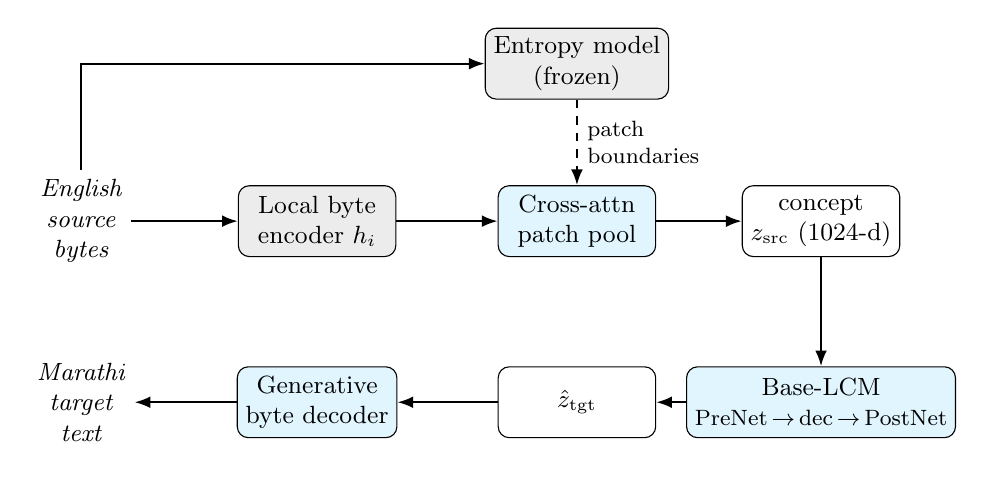
\begin{tikzpicture}[
    font=\small,
    box/.style={draw, rounded corners, minimum height=9mm, minimum width=20mm,
      align=center, inner sep=3pt},
    frozen/.style={box, fill=gray!15},
    train/.style={box, fill=cyan!12},
    io/.style={align=center, font=\small\itshape},
    ar/.style={-{Latex[length=2mm]}, thick},
    dar/.style={-{Latex[length=2mm]}, thick, dashed},
  ]
    % Top row: concept encoder (left -> right)
    \node[io]     (bytes) at (0,0)   {English\\source\\bytes};
    \node[frozen] (enc)   at (3,0)   {Local byte\\encoder $h_i$};
    \node[train]  (pool)  at (6.3,0) {Cross-attn\\patch pool};
    \node[box]    (zsrc)  at (9.4,0) {concept\\$z_{\text{src}}$ (1024-d)};
    \node[frozen] (ent)   at (6.3,2.0) {Entropy model\\(frozen)};
    % Bottom row: translate + decode (right -> left)
    \node[train]  (lcm)   at (9.4,-2.3) {Base-LCM\\{\footnotesize PreNet\,$\to$\,dec\,$\to$\,PostNet}};
    \node[box]    (ztgt)  at (6.3,-2.3) {$\hat z_{\text{tgt}}$};
    \node[train]  (dec)   at (3,-2.3)   {Generative\\byte decoder};
    \node[io]     (out)   at (0,-2.3)   {Marathi\\target\\text};
    % Encoder arrows
    \draw[ar]  (bytes) -- (enc);
    \draw[ar]  (enc)   -- (pool);
    \draw[ar]  (pool)  -- (zsrc);
    \draw[ar]  (bytes.north) |- (ent.west);
    \draw[dar] (ent)   -- node[right, align=left, font=\footnotesize]
                            {patch\\boundaries} (pool);
    % Connector + decode arrows
    \draw[ar]  (zsrc) -- (lcm);
    \draw[ar]  (lcm)  -- (ztgt);
    \draw[ar]  (ztgt) -- (dec);
    \draw[ar]  (dec)  -- (out);
  \end{tikzpicture}}
  \caption{\textbf{BLT-LCM pipeline.} English source bytes are encoded to per-byte
  hidden states $h_i$; a \emph{frozen} entropy model marks patch boundaries
  (dashed), and a cross-attention pooler aggregates each patch's hidden states
  into a 1024-d concept $z_{\text{src}}$. Base-LCM maps the source concept to a
  predicted target concept $\hat z_{\text{tgt}}$ (MSE), which a generative byte
  decoder renders into Marathi. Shaded blue modules are trained (pooler and
  decoder by byte reconstruction, the LCM by concept regression); gray modules
  are frozen. \textbf{Takeaway:} tokenization never enters the pipeline --
  concepts are built from pooled byte hidden states, not from a subword
  vocabulary or from the entropy model's logits.}
  \label{fig:arch}
\end{figure}

\paragraph{Byte encoding and entropy patching.}
Input text is encoded as UTF-8 bytes, offset by four reserved special-token ids (vocabulary size 260). A small byte-level causal Transformer (RoPE attention, SwiGLU FFN) is trained for next-byte prediction and used \emph{only} to place patch boundaries: following BLT, a new patch begins wherever the model's next-byte entropy exceeds a threshold $\tau$ (a global threshold tuned to a target average patch size; we use $\tau=1.335$ by default). This entropy model is never used as a source of concept features.

\paragraph{Cross-attention patch pooling.}
The same byte sequence is passed through the encoder backbone to obtain per-byte hidden states $h_i \in \mathbb{R}^{d}$ ($d=256$), with full-sentence context. For each patch, a Perceiver-style multi-headed cross-attention pools the patch's byte hidden states into a single patch representation: the query is initialized from the masked mean of the patch's hidden states and attends only to the bytes belonging to that patch (padding is masked out). Patch representations are averaged into a sentence-level concept vector. This follows the BLT principle that patch representations come from the local encoder's byte hidden states, not from the entropy model.

\begin{figure}[t]
  \centering
  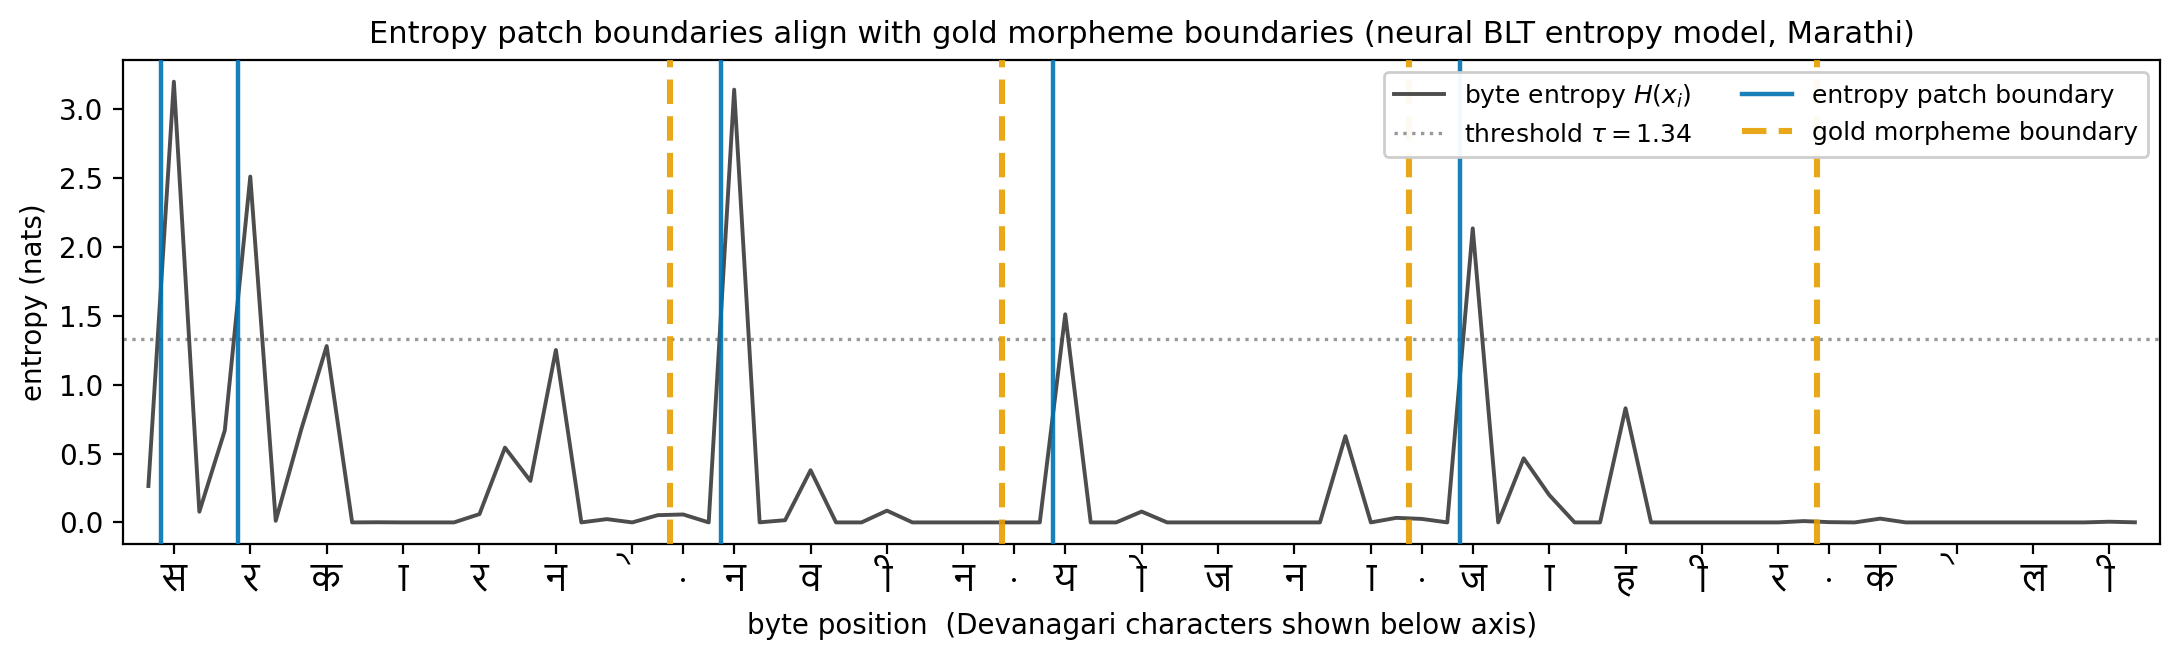
\includegraphics[width=\linewidth]{patch_morpheme_example.png}
  \caption{\textbf{Entropy patches track morphology.} Per-byte entropy of the
  neural BLT entropy model on a Marathi sentence, with entropy-based patch
  boundaries (solid blue, where $H(x_i)>\tau$) and gold morpheme boundaries from
  the Indic NLP unsupervised analyzer (dashed orange). Patch boundaries coincide
  with morpheme boundaries at every internal word/morpheme transition that the
  analyzer marks (within $\pm2$ bytes), with one boundary whose entropy stays
  just below $\tau$ (a miss). \textbf{Takeaway:} because morpheme onsets raise
  next-byte uncertainty in an agglutinative script, entropy patching segments
  the byte stream along linguistic units without any vocabulary. Aggregate
  boundary-F1 across thresholds is reported in the alignment study.}
  \label{fig:align}
\end{figure}

\paragraph{Concept-level translation with the LCM.}
The LCM is a pre-net / Transformer-decoder / post-net regressor (as in Base-LCM): the pre-net normalizes and projects a concept into the model width, decoder layers attend to the source concept as cross-attention memory, and the post-net projects back to the concept dimension. For translation, the source (English) concept is the memory and the model predicts the target (Marathi) concept, trained with a mean-squared-error objective between the predicted and reference target concepts.

\paragraph{Generative decoding.}
A predicted target concept is turned back into Marathi text by a trained autoregressive byte decoder that cross-attends to the concept and generates UTF-8 bytes greedily until an end-of-text token. The cross-attention pooler and this decoder are trained jointly with a byte-reconstruction objective while the entropy backbone (and hence the patch boundaries) stay frozen, so the boundaries used for analysis never drift during training. Decoding is generative; nearest-neighbor retrieval over a sentence bank is reported only as a baseline.

\section{Theoretical Analysis}
\label{sec:theory}

We give an informal scaling argument -- a heuristic motivation under explicit assumptions, not a theorem -- for why byte-level entropy patching should reduce concept encoding error for high-fertility words, and then validate the resulting relationship empirically (Section~\ref{sec:experiments}).

\paragraph{Setup and assumptions.}
Consider a word $w$ with fertility $\lambda$ (its number of morphemes), and let $E(w)$ denote the concept encoding error incurred for $w$. We assume: (A1) error is dominated by segmentation units that straddle morpheme boundaries, so $E$ grows with the number of boundary-violating segments $m(w)$; (A2) to first order $E(w) \approx \kappa\, m(w)$ for an encoder-independent constant $\kappa$; (A3) a BPE vocabulary tuned on a high-resource language fragments $w$ into $m_{\mathrm{BPE}}(w) = \Theta(\lambda)$ morphologically unaligned pieces, because subword frequencies do not track the morpheme inventory of a low-resource agglutinative language; and (A4) entropy patching places boundaries preferentially where next-byte entropy spikes, which for agglutinative morphology tends to coincide with morpheme boundaries (Figure~\ref{fig:align}), so BLT's boundary-violating count grows sublinearly, $m_{\mathrm{BLT}}(w) = \Theta(\lambda^{\,1-\alpha})$ for some $\alpha \in (0,1]$ measuring how well entropy tracks morphology.

\paragraph{Resulting relationship.}
Combining (A2)--(A4),
\[
\frac{E_{\mathrm{BLT}}(w)}{E_{\mathrm{BPE}}(w)} \;=\; \frac{m_{\mathrm{BLT}}(w)}{m_{\mathrm{BPE}}(w)} \;=\; \Theta\!\left(\lambda^{-\alpha}\right),
\qquad\text{so, up to constants,}\qquad E_{\mathrm{BLT}} \;\le\; \lambda^{-\alpha}\, E_{\mathrm{BPE}}.
\]
The exponent $\alpha$ is \emph{not} derived from first principles: it is the degree to which entropy boundaries align with morphology, and we estimate it from data rather than assume it. At $\alpha=0$ (entropy carries no morphological signal) the two encoders are on par; larger $\alpha$ predicts a larger BLT advantage for higher-fertility words.

\paragraph{What we do and do not claim.}
This is a scaling heuristic under strong assumptions (A1--A4), not a proof: $E$ is a proxy, $\kappa$ is assumed shared across encoders, and the $\Theta$ orders hide constants. We therefore treat $E_{\mathrm{BLT}} \le \lambda^{-\alpha} E_{\mathrm{BPE}}$ as an empirical diagnostic and test it per morpheme class, reporting the fraction of classes that satisfy it and the correlation between $\lambda$ and the measured chrF++ gain.

\section{Experiments}
\label{sec:experiments}

\paragraph{Data and task.}
We use the BhashaSetu English--Marathi parallel corpus. The task is English$\rightarrow$Marathi sentence translation. We train on deterministic shuffled fractions of the corpus (25\%, 50\%, 80\%) to probe data efficiency, holding out a fixed evaluation set.

\paragraph{Baselines.}
We compare BLT-LCM against a SONAR-LCM model (the same LCM over a SONAR-like byte encoder with a fixed-size bottleneck) and BPE-based systems: a from-scratch BPE encoder--decoder Transformer, a BPE-LCM, and a LoRA/QLoRA-fine-tuned BPE Llama-8B.

\paragraph{Metrics and robustness.}
We report BLEU, chrF++, and TER (sacreBLEU), METEOR (NLTK), and COMET (Unbabel), computed on generated Marathi. Robustness is measured by applying character-level noise (missing matras and script-appropriate substitutions) to the source at 0\%, 10\%, and 20\% and re-scoring.

\paragraph{Linguistic analyses.}
We additionally report (i) precision/recall/F1 of entropy patch boundaries against gold morpheme segmentations as a function of $\tau$, (ii) a fixed-length chunking ablation (4- and 8-byte patches) to isolate the effect of entropy-adaptivity from byte-level modeling alone, (iii) fertility ($\lambda$) by morpheme class, and (iv) the correlation between $\lambda$ and per-class chrF++ gain.

\section{Results}

% RESULTS PENDING: fill the tables/figures below from the metric CSVs produced by
% the training/eval scripts (results/blt_lcm_mt_*.csv, morpheme_alignment/, etc.).
% Do not report numbers that have not been produced by an experiment run.
Results tables and figures are populated from the metric CSVs emitted by the training and evaluation scripts; the main comparison reports translation quality and noise robustness across data fractions, alongside the morpheme-alignment and fertility analyses.

\section{Ablation Studies}

\section{Discussion}

\section{Conclusion}

\bibliography{references}


%%%%%%%%%%%%%%%%%%%%%%%%%%%%%%%%%%%%%%%%%%%%%%%%%%%%%%%%%%%%

\appendix

\section{Technical appendices and supplementary material}
Technical appendices with additional results, figures, graphs, and proofs may be submitted with the paper submission before the full submission deadline (see above). You can upload a ZIP file for videos or code, but do not upload a separate PDF file for the appendix. There is no page limit for the technical appendices. 

Note: Think of the appendix as ``optional reading'' for reviewers. The paper must be able to stand alone without the appendix; for example, adding critical experiments that support the main claims to an appendix is inappropriate. 

%%%%%%%%%%%%%%%%%%%%%%%%%%%%%%%%%%%%%%%%%%%%%%%%%%%%%%%%%%%%

\newpage
% Minimal NeurIPS checklist placeholder to allow CI builds.
% Replace the items below with the real checklist content before final submission.
\section*{Checklist}
\begin{enumerate}
  \item This is a placeholder checklist file added to allow the LaTeX build to succeed in CI.
  \item Replace or expand this file with the official NeurIPS checklist contents as needed.
\end{enumerate}


\end{document}